% Portfolio construction and simulation, one trading day of the backtest (bgarch.portfolio.portfolio ->
% src.portfolio.simulate_portfolio). Row d of a forecast file uses returns up to close d-1; its weight is
% executed at close d and held over close d -> close d+1.
\documentclass[tikz,border=3pt]{standalone}
% Shared look for the narrative diagrams (included by portfolio_flowchart.tex and rolling_design.tex)
\usepackage[T1]{fontenc}
\usepackage{lmodern}
\usepackage{amsmath,amssymb}
\renewcommand{\familydefault}{\sfdefault}
\usetikzlibrary{positioning,arrows.meta,calc,fit,backgrounds,decorations.pathreplacing}
\definecolor{ink}{HTML}{1F1F1E}
\definecolor{muted}{HTML}{6B6A63}
\definecolor{fc}{HTML}{2A78D6}   % statistical forecasting
\definecolor{al}{HTML}{EB6834}   % portfolio allocation
\definecolor{ex}{HTML}{1BAF7A}   % execution and accounting
\definecolor{ev}{HTML}{7A5BB5}   % performance evaluation
\definecolor{rule}{HTML}{D9D7CF}
\tikzset{
  box/.style={draw=#1, fill=#1!9, line width=0.8pt, rounded corners=3pt, align=flush left,
              inner sep=3.2pt, text=ink, font=\small},
  step/.style={box=#1, text width=3.75cm, minimum height=1.45cm},
  arr/.style={-{Stealth[length=2.4mm]}, line width=0.9pt, draw=muted},
  num/.style={circle, fill=#1, text=white, font=\scriptsize\bfseries, inner sep=1.2pt, minimum size=4mm},
}

\begin{document}
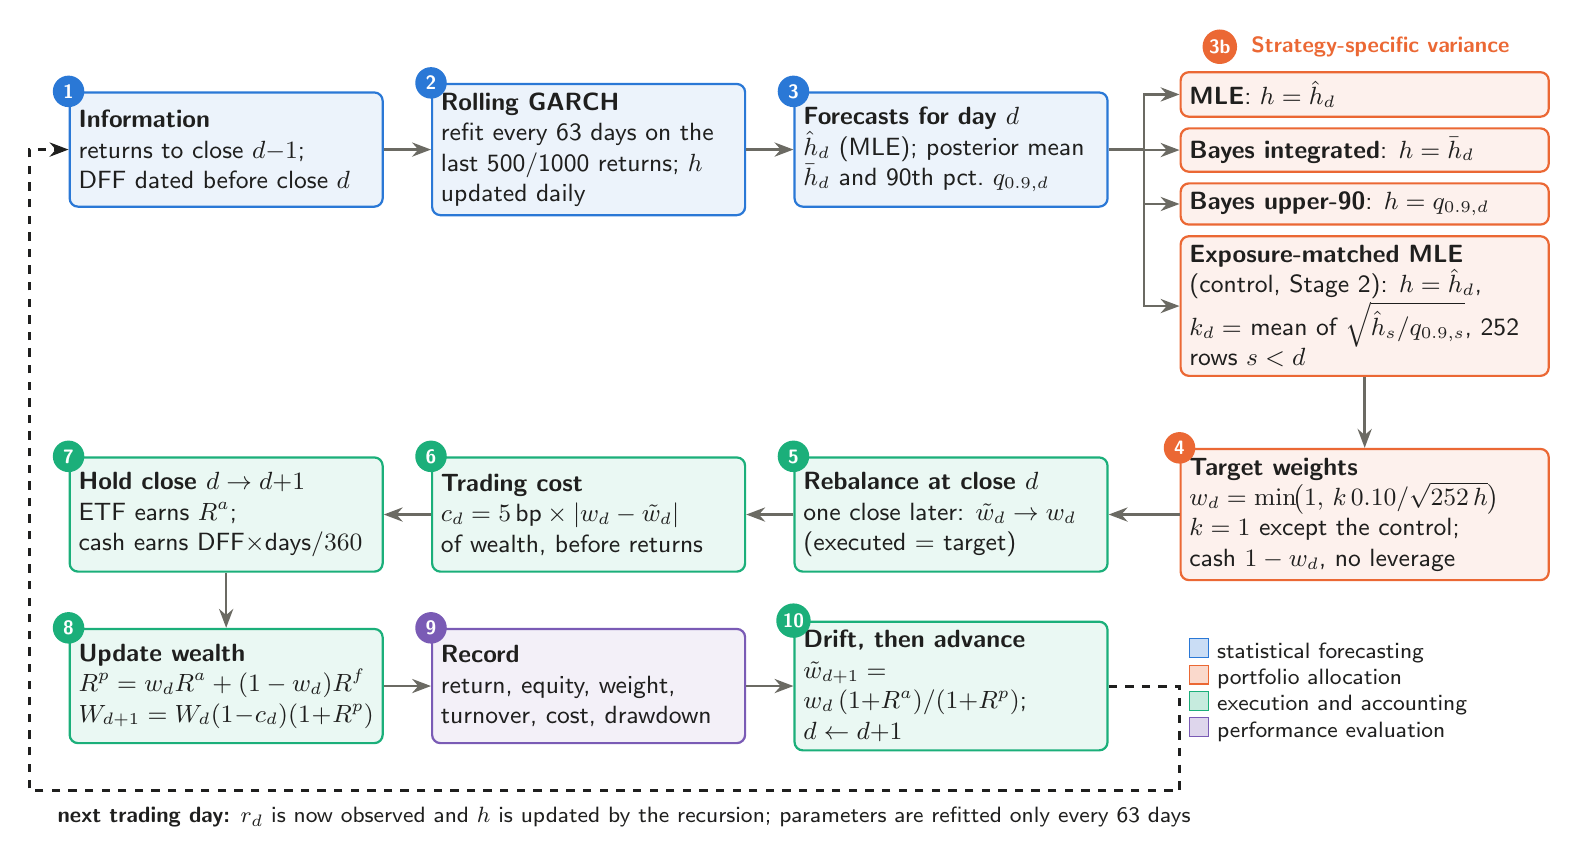
\begin{tikzpicture}[node distance=4mm and 5mm]
% ---------------- row 1: forecasting (left to right)
\node[step=fc] (s1) {\textbf{Information}\\ returns to close $d{-}1$;\\ DFF dated before close $d$};
\node[step=fc, right=6mm of s1] (s2) {\textbf{Rolling GARCH}\\ refit every 63 days on the last 500/1000 returns; $h$ updated daily};
\node[step=fc, right=6mm of s2] (s3) {\textbf{Forecasts for day $d$}\\ $\hat h_d$ (MLE); posterior mean $\bar h_d$ and 90th pct.\ $q_{0.9,d}$};
% ---------------- strategy branch (allocation)
\node[box=al, text width=4.45cm, right=9mm of s3, yshift=7mm] (b1) {\textbf{MLE}: $h=\hat h_d$};
\node[box=al, text width=4.45cm, below=1.2mm of b1] (b2) {\textbf{Bayes integrated}: $h=\bar h_d$};
\node[box=al, text width=4.45cm, below=1.2mm of b2] (b3) {\textbf{Bayes upper-90}: $h=q_{0.9,d}$};
\node[box=al, text width=4.45cm, below=1.2mm of b3] (b4) {\textbf{Exposure-matched MLE} (control, Stage 2): $h=\hat h_d$, $k_d=$ mean of $\sqrt{\hat h_s/q_{0.9,s}}$, 252 rows $s<d$};
\node[font=\footnotesize\bfseries, text=al, above=0.6mm of b1, xshift=2mm] (blab) {Strategy-specific variance};
% ---------------- row 2: allocation + execution (right to left)
\node[step=al, below=9mm of b4.south, anchor=north, text width=4.45cm] (s4) {\textbf{Target weights}\\
  $w_d=\min\!\bigl(1,\,k\,0.10/\sqrt{252\,h}\bigr)$\\ $k=1$ except the control;\\ cash $1-w_d$, no leverage};
\node[step=ex] (s5) at (s3 |- s4) {\textbf{Rebalance at close $d$}\\ one close later: $\tilde w_d\to w_d$\\ (executed $=$ target)};
\node[step=ex] (s6) at (s2 |- s4) {\textbf{Trading cost}\\ $c_d=5\,\text{bp}\times|w_d-\tilde w_d|$\\ of wealth, before returns};
\node[step=ex] (s7) at (s1 |- s4) {\textbf{Hold close $d\to d{+}1$}\\ ETF earns $R^{a}$;\\ cash earns DFF$\times$days$/360$};
% ---------------- row 3: accounting + evaluation (left to right)
\node[step=ex, below=7mm of s7] (s8) {\textbf{Update wealth}\\ $R^{p}=w_dR^{a}+(1-w_d)R^{f}$\\ $W_{d+1}=W_d(1-c_d)(1+R^{p})$};
\node[step=ev] (s9) at (s8 -| s6) {\textbf{Record}\\ return, equity, weight,\\ turnover, cost, drawdown};
\node[step=ex] (s10) at (s8 -| s5) {\textbf{Drift, then advance}\\ $\tilde w_{d+1}=w_d\,(1{+}R^{a})/(1{+}R^{p})$;\\ $d\leftarrow d{+}1$};
% ---------------- step numbers
\node[num=fc] at (s1.north west) {1}; \node[num=fc] at (s2.north west) {2}; \node[num=fc] at (s3.north west) {3};
\node[num=al, left=0.5mm of blab] {3b};
\node[num=al] at (s4.north west) {4}; \node[num=ex] at (s5.north west) {5}; \node[num=ex] at (s6.north west) {6};
\node[num=ex] at (s7.north west) {7}; \node[num=ex] at (s8.north west) {8}; \node[num=ev] at (s9.north west) {9};
\node[num=ex] at (s10.north west) {10};
% ---------------- arrows
\draw[arr] (s1) -- (s2); \draw[arr] (s2) -- (s3);
\draw[arr] (s3.east) -- ++(4.5mm,0) |- (b1.west); \draw[arr] (s3.east) ++(4.5mm,0) |- (b2.west);
\draw[arr] (s3.east) ++(4.5mm,0) |- (b3.west); \draw[arr] (s3.east) ++(4.5mm,0) |- (b4.west);
\draw[arr] (b4) -- (s4);
\draw[arr] (s4) -- (s5); \draw[arr] (s5) -- (s6); \draw[arr] (s6) -- (s7);
\draw[arr] (s7) -- (s8); \draw[arr] (s8) -- (s9); \draw[arr] (s9) -- (s10);
% loop back: next trading day
\draw[arr, draw=ink, line width=1.1pt, dashed] (s10.east) -- ++(9mm,0) coordinate (lp)
   -- (lp |- s10.south) -- ++(0,-5mm) coordinate (lq) -- (lq -| s1.west) -- ++(-5mm,0) coordinate (lr)
   -- (lr |- s1.west) -- (s1.west);
\node[font=\footnotesize, text=ink, align=center, below=0.8mm] at ($(lq)!0.5!(lq -| s1.west)$)
   {\textbf{next trading day:} $r_d$ is now observed and $h$ is updated by the recursion; parameters are refitted only every 63 days};
% ---------------- legend (bottom right)
\node[anchor=north west, font=\footnotesize, align=left, text=ink] (leg) at ($(s4.south west)+(0,-6mm)$) {%
  \tikz\fill[fc!25,draw=fc] (0,0) rectangle (2.4mm,2.4mm); statistical forecasting\\
  \tikz\fill[al!25,draw=al] (0,0) rectangle (2.4mm,2.4mm); portfolio allocation\\
  \tikz\fill[ex!25,draw=ex] (0,0) rectangle (2.4mm,2.4mm); execution and accounting\\
  \tikz\fill[ev!25,draw=ev] (0,0) rectangle (2.4mm,2.4mm); performance evaluation};
\end{tikzpicture}
\end{document}
